\section{Конструкторская часть}

\subsection{Основной алгоритм}

На Рисунке \ref{fig200:image} приведен основной алгоритм работы Bittorrent-клиента.
\begin{figure}[h]
	\begin{center}
		{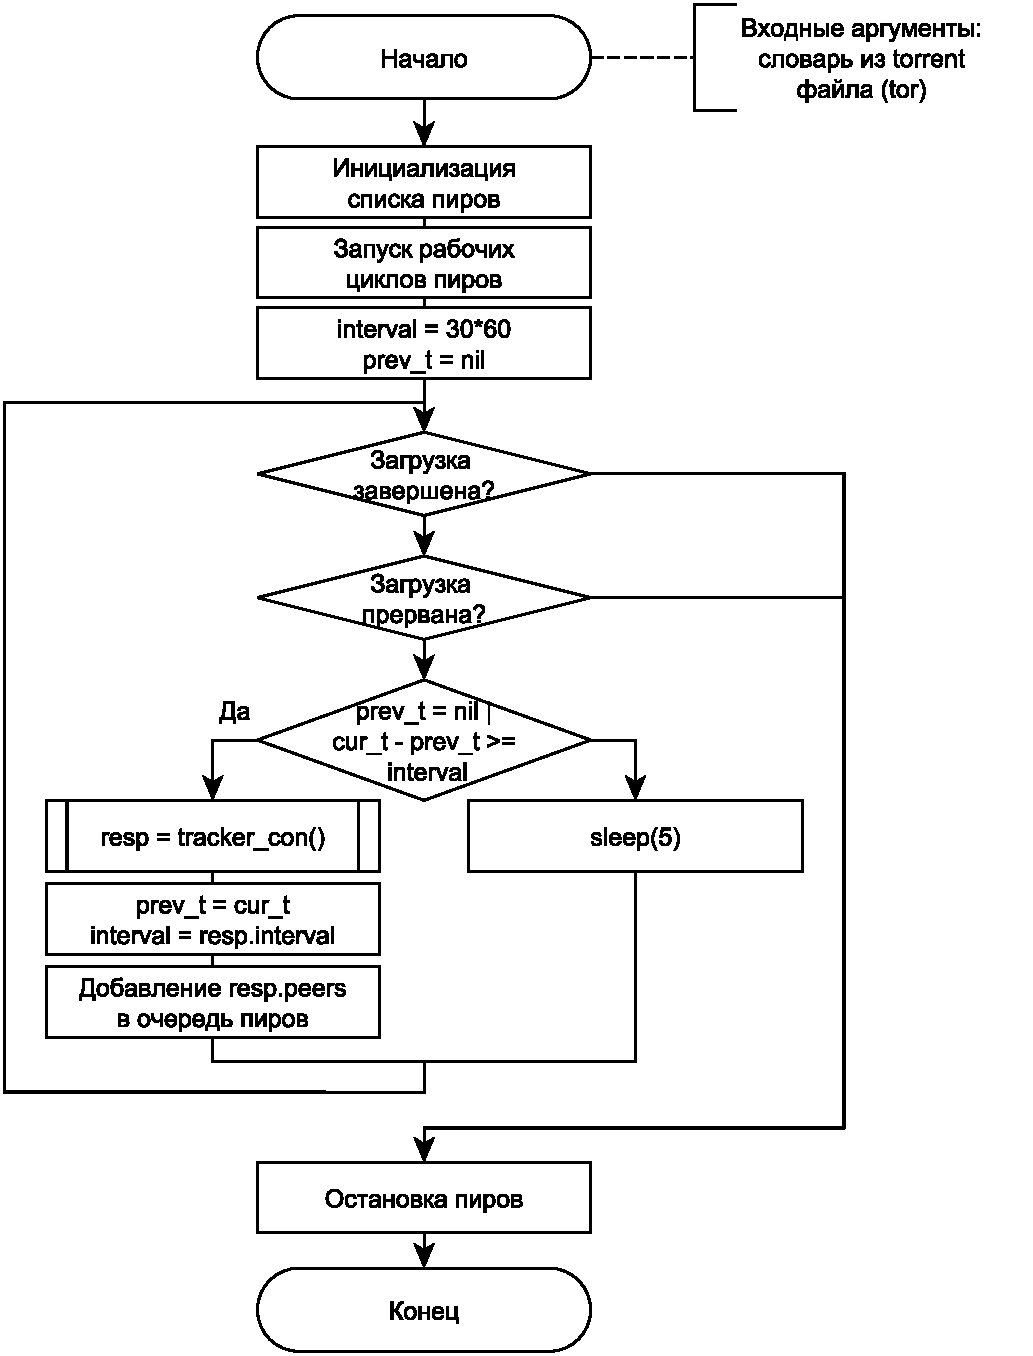
\includegraphics[scale = 0.75]{img/main.pdf}}
		\caption{Основной алгоритм}
		\label{fig200:image}
	\end{center}
\end{figure}

\newpage

\subsection{Алгоритм взаимодействия с сервером}
Детали алгоритма взаимодействия с сервером продемонстрированы на схеме \ref{fig201:image}.
\begin{figure}[h]
	\begin{center}
		{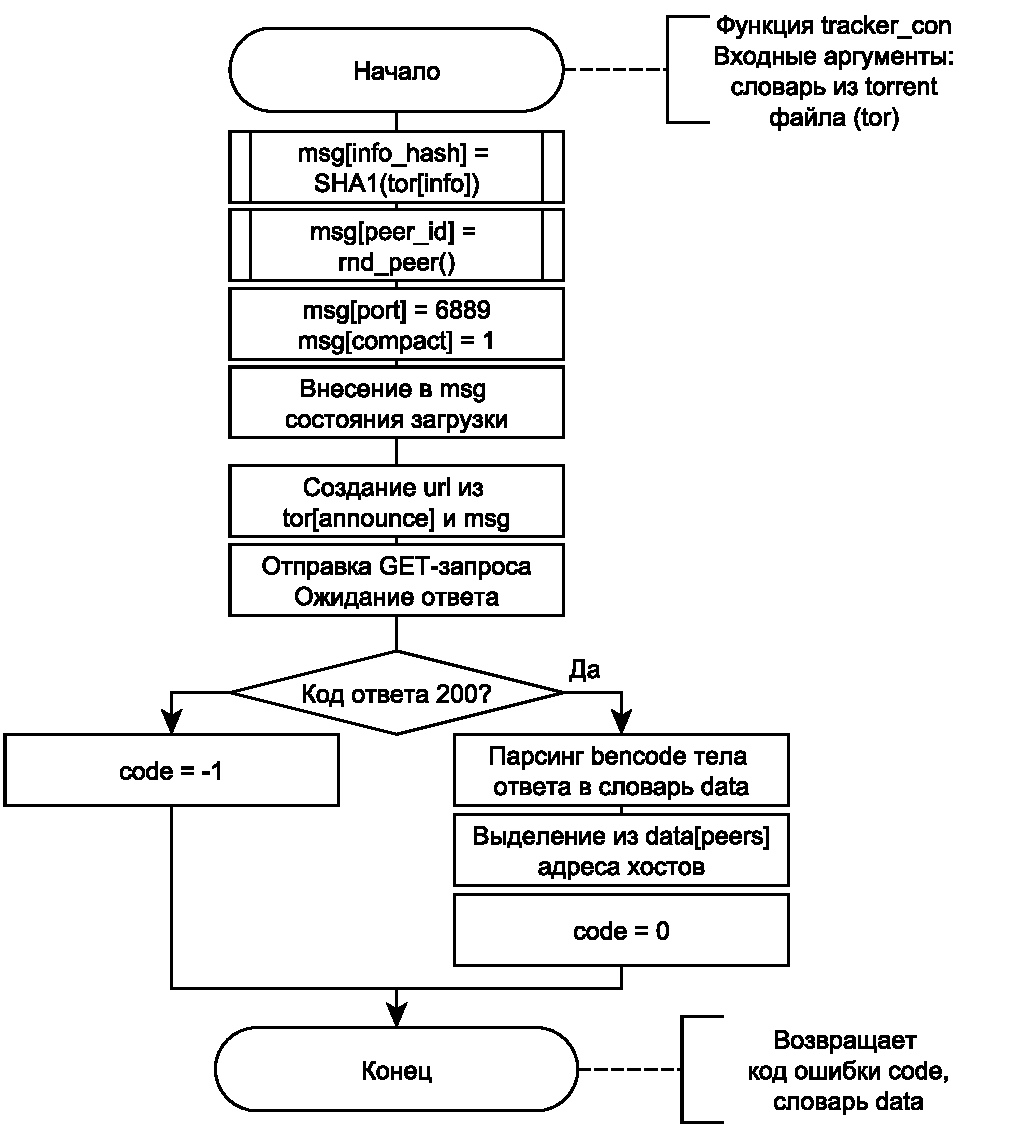
\includegraphics[scale = 0.75]{img/server.pdf}}
		\caption{Алгоритм взаимодействия с сервером}
		\label{fig201:image}
	\end{center}
\end{figure}

\newpage

\subsection{Алгоритм рукопожатия}
Этот алгоритм приведён на Рисунке \ref{fig202:image}.
\begin{figure}[h]
	\begin{center}
		{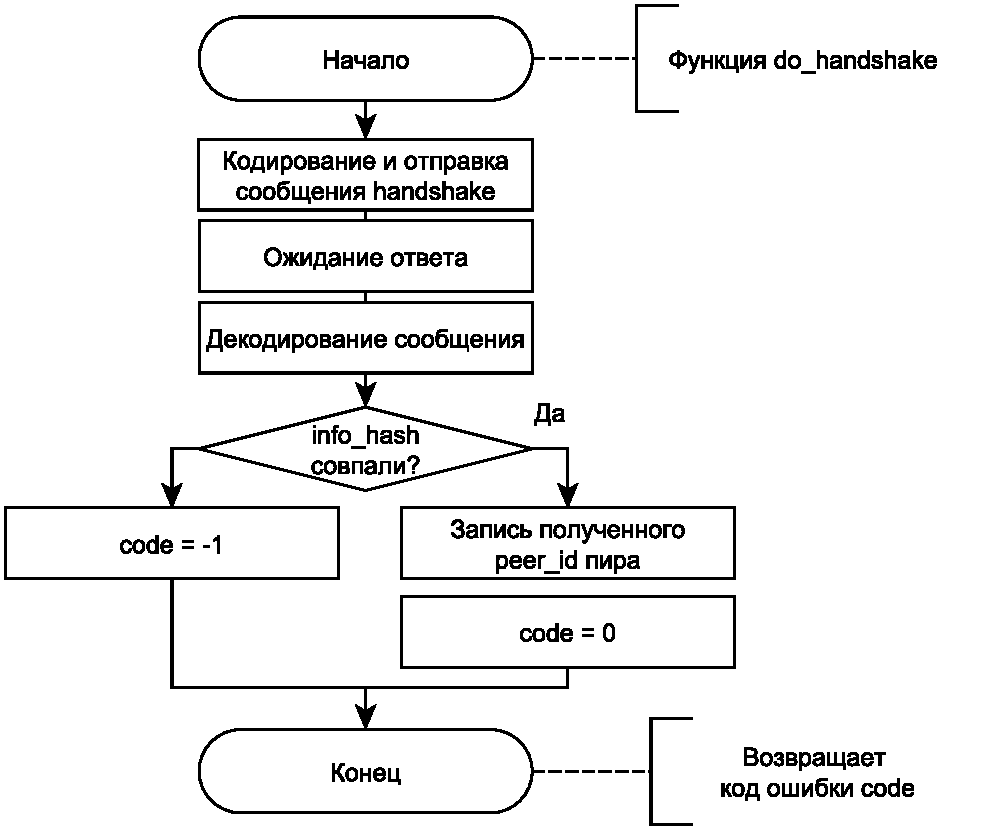
\includegraphics[scale = 0.75]{img/handshake.pdf}}
		\caption{Алгоритм рукопожатия}
		\label{fig202:image}
	\end{center}
\end{figure}

\newpage

\subsection{Алгоритм взаимодействия с пирами}
Детали взаимодействия с пирами приведены ниже, на Рисунке \ref{fig203:image}.
\begin{figure}[h]
	\begin{center}
		{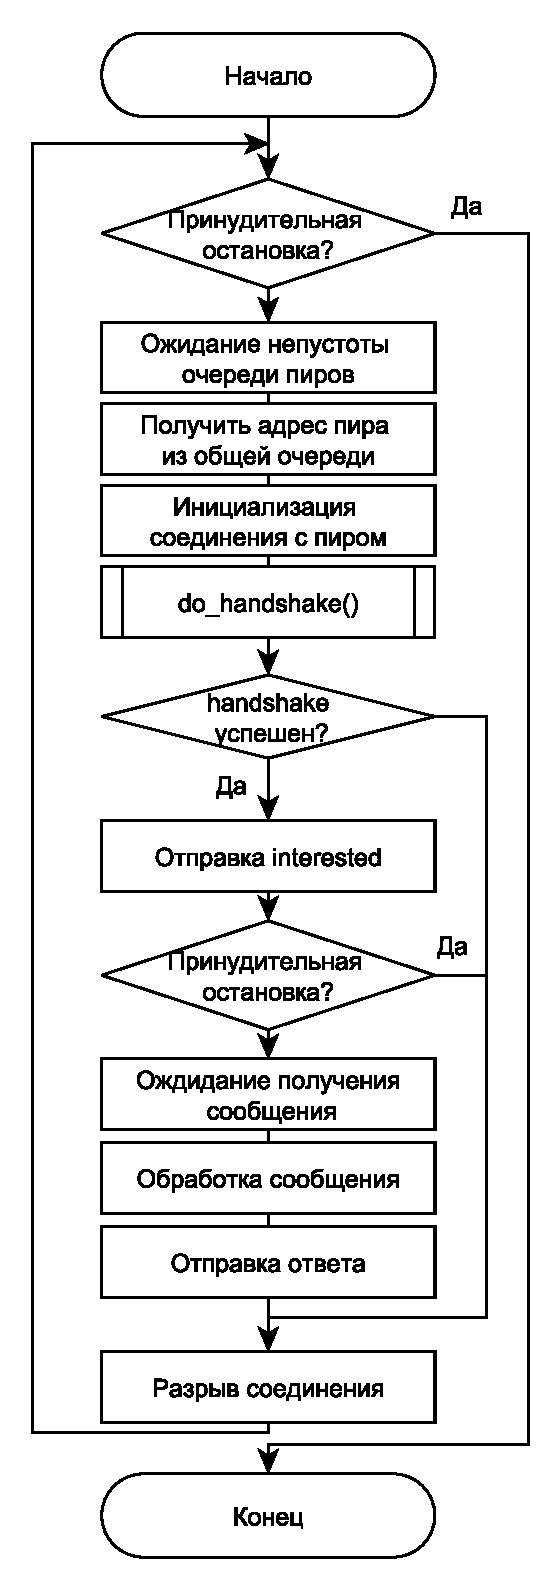
\includegraphics[scale = 0.7]{img/peer.pdf}}
		\caption{Алгоритм взаимодействия с пирами}
		\label{fig203:image}
	\end{center}
\end{figure}